\documentclass[mathserif]{beamer}
\usepackage[english,russian]{babel}
\usepackage[utf8]{inputenc}
\usepackage{amsmath}
\usetheme{Warsaw}
\usepackage{listings}
\usepackage{xcolor}
\usepackage{tikz}
\usetikzlibrary{graphs}

\lstset{
    frame=tb,
    tabsize=4,
    showstringspaces=false,
    numbers=left,
    commentstyle=\color{green},
    keywordstyle=\color{blue},
    stringstyle=\color{red},
    emph={baz},
    emphstyle=\textbf
}

\begin{document}

\title{SAT/SMT solvers\newline  1. Introduction}
\author{Roman Kholin}
\institute{Lalambda}
\date{Tbilisi, 2023}

\begin{frame}
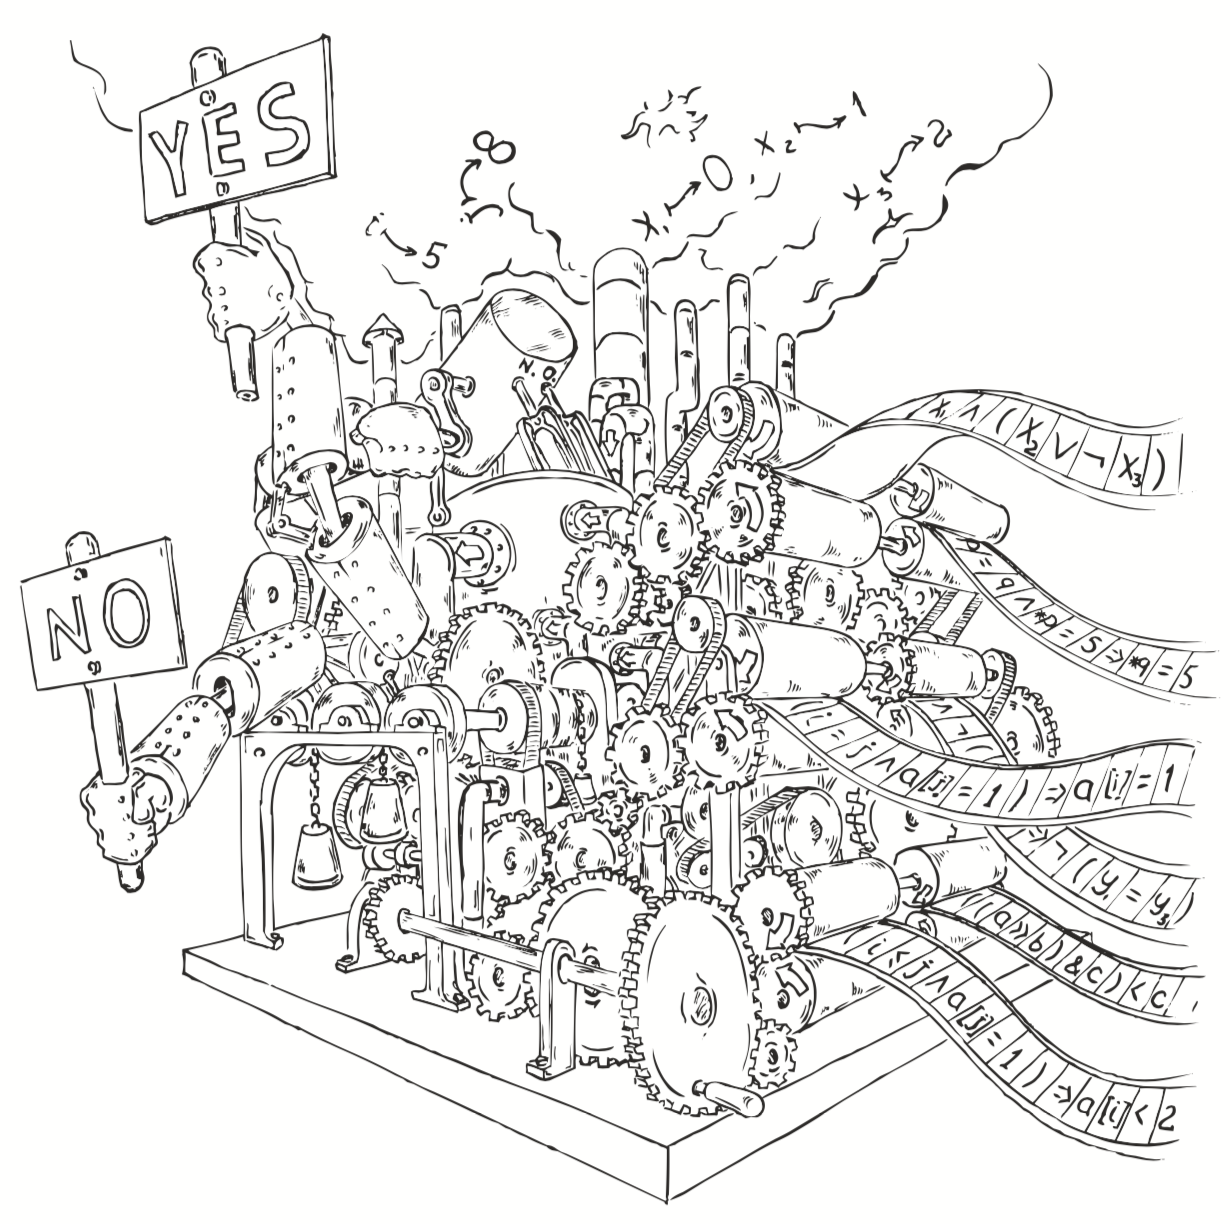
\includegraphics[scale=0.5]{../decision-procedure.png}
\end{frame}

\frame{\titlepage}

\begin{frame}{Outline}
\begin{itemize}
\item What are SAT and SMT
\item How they are made
\item Where to use they
\end{itemize}
\end{frame}

\begin{frame}
Edmund Clarke:
\begin{block}{}
A key technology of the 21st century
\end{block}
Donald Knuth
\begin{block}{}
Evidently a killer app, because it is key to the solution of so mane other problems
\end{block}
\end{frame}

\begin{frame}{Examples}
You are the chief of protocol and you make a diner for an ambassadors. The prince wants to invite either an ambassador from Peru or not to invite ambassador from Qatar. The queen wants to see the ambassadors of Qatar or Romania. The king does not want to see ambassadors from Romania or Peru. Whom to invite for dinner?
\end{frame}

\begin{frame}{Examples}
\begin{itemize}
\item The set of natural numbers was divided into subsets. Does any contain Pythagorean triple?
\item Let's the number of subsets is three and original set is $\{1, \dots, N\}$. The minimal $N$ such that it can't be diveded is 7825
\item There is no answer for number of subsets 3. It's could be shown that $\{1, \dots, 10^7\}$ could be diveded
\end{itemize}
\end{frame}

\begin{frame}{Examples}
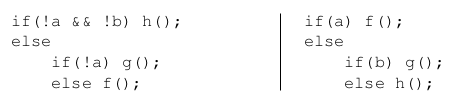
\includegraphics[scale=0.5]{equivalent1.png}
\end{frame}

\begin{frame}{Examples}
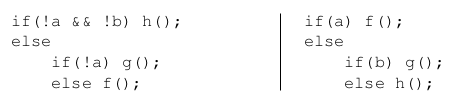
\includegraphics[scale=0.5]{equivalent1.png}
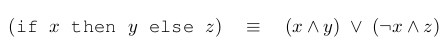
\includegraphics[scale=0.5]{equivalent2.png}
\end{frame}

\begin{frame}{Examples}
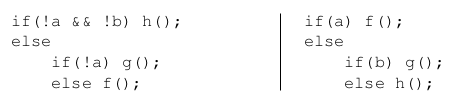
\includegraphics[scale=0.5]{equivalent1.png}
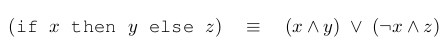
\includegraphics[scale=0.5]{equivalent2.png}
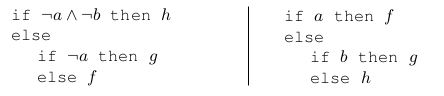
\includegraphics[scale=0.5]{equivalent3.png}
\end{frame}

\begin{frame}{Examples}
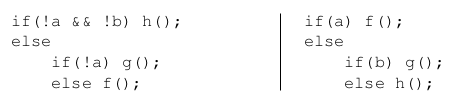
\includegraphics[scale=0.5]{equivalent1.png}
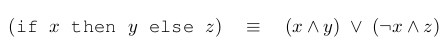
\includegraphics[scale=0.5]{equivalent2.png}
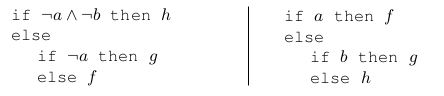
\includegraphics[scale=0.5]{equivalent3.png}
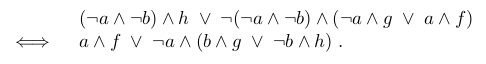
\includegraphics[scale=0.5]{equivalent4.png}
\end{frame}

\begin{frame}{Definitions}
\begin{block}{Propositional formula}
Given a set $V$, brackets, $\vee$, $\wedge$, $\rightarrow$, $\lnot$, let define an formulas as:
\begin{itemize}
\item all variables $V$ are formula.
\item if $A$ is formula, then $\lnot(A)$ - fromula
\item if $A$, $B$ are formulas, then $(A)\vee(B)$, $(A)\wedge(B)$, $(A)\rightarrow(B)$ is formula.
\end{itemize}
\end{block}
\begin{block}{Assignment}
Given a formula $\varphi$, an $assignment$ of $\varphi$ from a domain $D$ is a function mapping $\varphi$ 's variables to elements of $D$. An assignment to $\varphi$ is full if all of $\varphi$ 's variables are assigned, and partial otherwise.
\end{block}
\end{frame}

\begin{frame}{Definitions}
\begin{block}{Satisfiability, Validity, and Contradiction}
\begin{itemize}
\item A formula is $satisfiable$ if there exists an assignment of its variables under which the formula evaluates to true.
\item A formula is a $contradiction$ if it is not $satisfiable$.
\item A formula is $valid$ (also called a $tautology$) if it evaluates to true under all assignments.
\end{itemize}
\end{block}
\begin{block}{The decision problem for formulas}
The decision problem for a given formula $\varphi$ is to determine whether $\varphi$ is valid.
\end{block}
\begin{block}{Soundness of a procedure}
A procedure for a decision problem is sound if, when it returns $Valid$, the input formula is $valid$.
\end{block}
\end{frame}

\begin{frame}{Definitions}
\begin{block}{Completeness of a procedure}
A procedure for a decision problem is $complete$ if
\begin{itemize}
\item it always terminates, and
\item it returns $Valid$ when the input formula is valid
\end{itemize}
\end{block}
\begin{block}{Decision procedure}
A procedure is called a decision procedure for $T$ if it is sound and complete with respect to every formula of $T$
\end{block}
\begin{block}{Decidability of a theory}
A theory is decidable if and only if there is a decision procedure for it
\end{block}
\end{frame}

\begin{frame}{Definitions}
\begin{block}{Negation Normal Form (NNF)}
A formula is in negation normal form (NNF) if negation is allowed only over variables, and $\vee$, $\wedge$, $\lnot$ are the only allowed Boolean connectives
\end{block}
\begin{block}{Literal}
A $literal$ is either an variable or its negation. We say that a literal is negative if it is a negated variable, and positive otherwise
\end{block}
\begin{block}{State of a literal under an assignment}
A positive literal is satisfied if its variable is assigned TRUE. Similarly, a negative literal is satisfied if its variable is assigned FALSE
\end{block}
\end{frame}

\begin{frame}{Definitions}
\begin{block}{Monotonicity of NNF}
Let $\varphi$ be a formula in NNF and let $\alpha$ be an assignment of its variables.
Let the positive set of $\alpha$ with respect to $\varphi$, denoted $pos(\alpha, \varphi)$, be the literals that are satisfied by $\alpha$.
For every assignment $\alpha'$ to $\varphi$'s variables such that $pos(\alpha, \varphi) \subseteq pos(\alpha', \varphi), \alpha \models \varphi \rightarrow \alpha' \models \varphi$
\end{block}
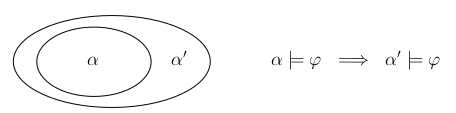
\includegraphics[scale=0.5]{monotonicity.png}
\end{frame}

\begin{frame}{Definitions}
\begin{block}{Disjunctive Normal Form (DNF)}
A formula is in disjunctive normal form if it is a disjunction of conjunctions of literals, i.e., a formula of the form $\bigvee\limits_{i}\bigwedge\limits_{j}l_{ij}$, where $l_{ij}$ is the $j$-th literal in the $i$-th term (a term is a conjunction of literals)
\end{block}
\begin{block}{Conjunctive Normal Form (CNF)}
A formula is in conjunctive normal form if it is a conjunction of disjunctions of literals, i.e., it has the form $\bigwedge\limits_{i}\bigvee\limits{j}l_{ij}$, where $l_{ij}$ is the $j$-th literal in the $i$-th clause (a clause is a disjunction of literals)
\end{block}
\end{frame}

\begin{frame}{Tseitin Transformation}
$\phi := ((p \vee q) \wedge r) \rightarrow (\lnot s)$
\begin{block}{Equisatisfiability}
Two formulas are equisatisfiable if they are both satisfiable or they are both unsatisfiable
\end{block}
\end{frame}

\begin{frame}{SAT}
\begin{block}{}
Given a propositional formula f over n propositional variables $V = {x_1, \dots, x_n}$, is there are an assignment $\alpha: V \rightarrow \{0, 1\}$ with $\alpha(f) = 1$?
\end{block}
\end{frame}

\begin{frame}{SAT}
\begin{block}{}
Given a propositional formula f over n propositional variables $V = {x_1, \dots, x_n}$, is there are an assignment $\alpha: V \rightarrow \{0, 1\}$ with $\alpha(f) = 1$?
\end{block}
\begin{itemize}
\item SAT belongs to NP (for n > 2)
\item SAT is complete for NP
\end{itemize}
\end{frame}

\begin{frame}{Examples}
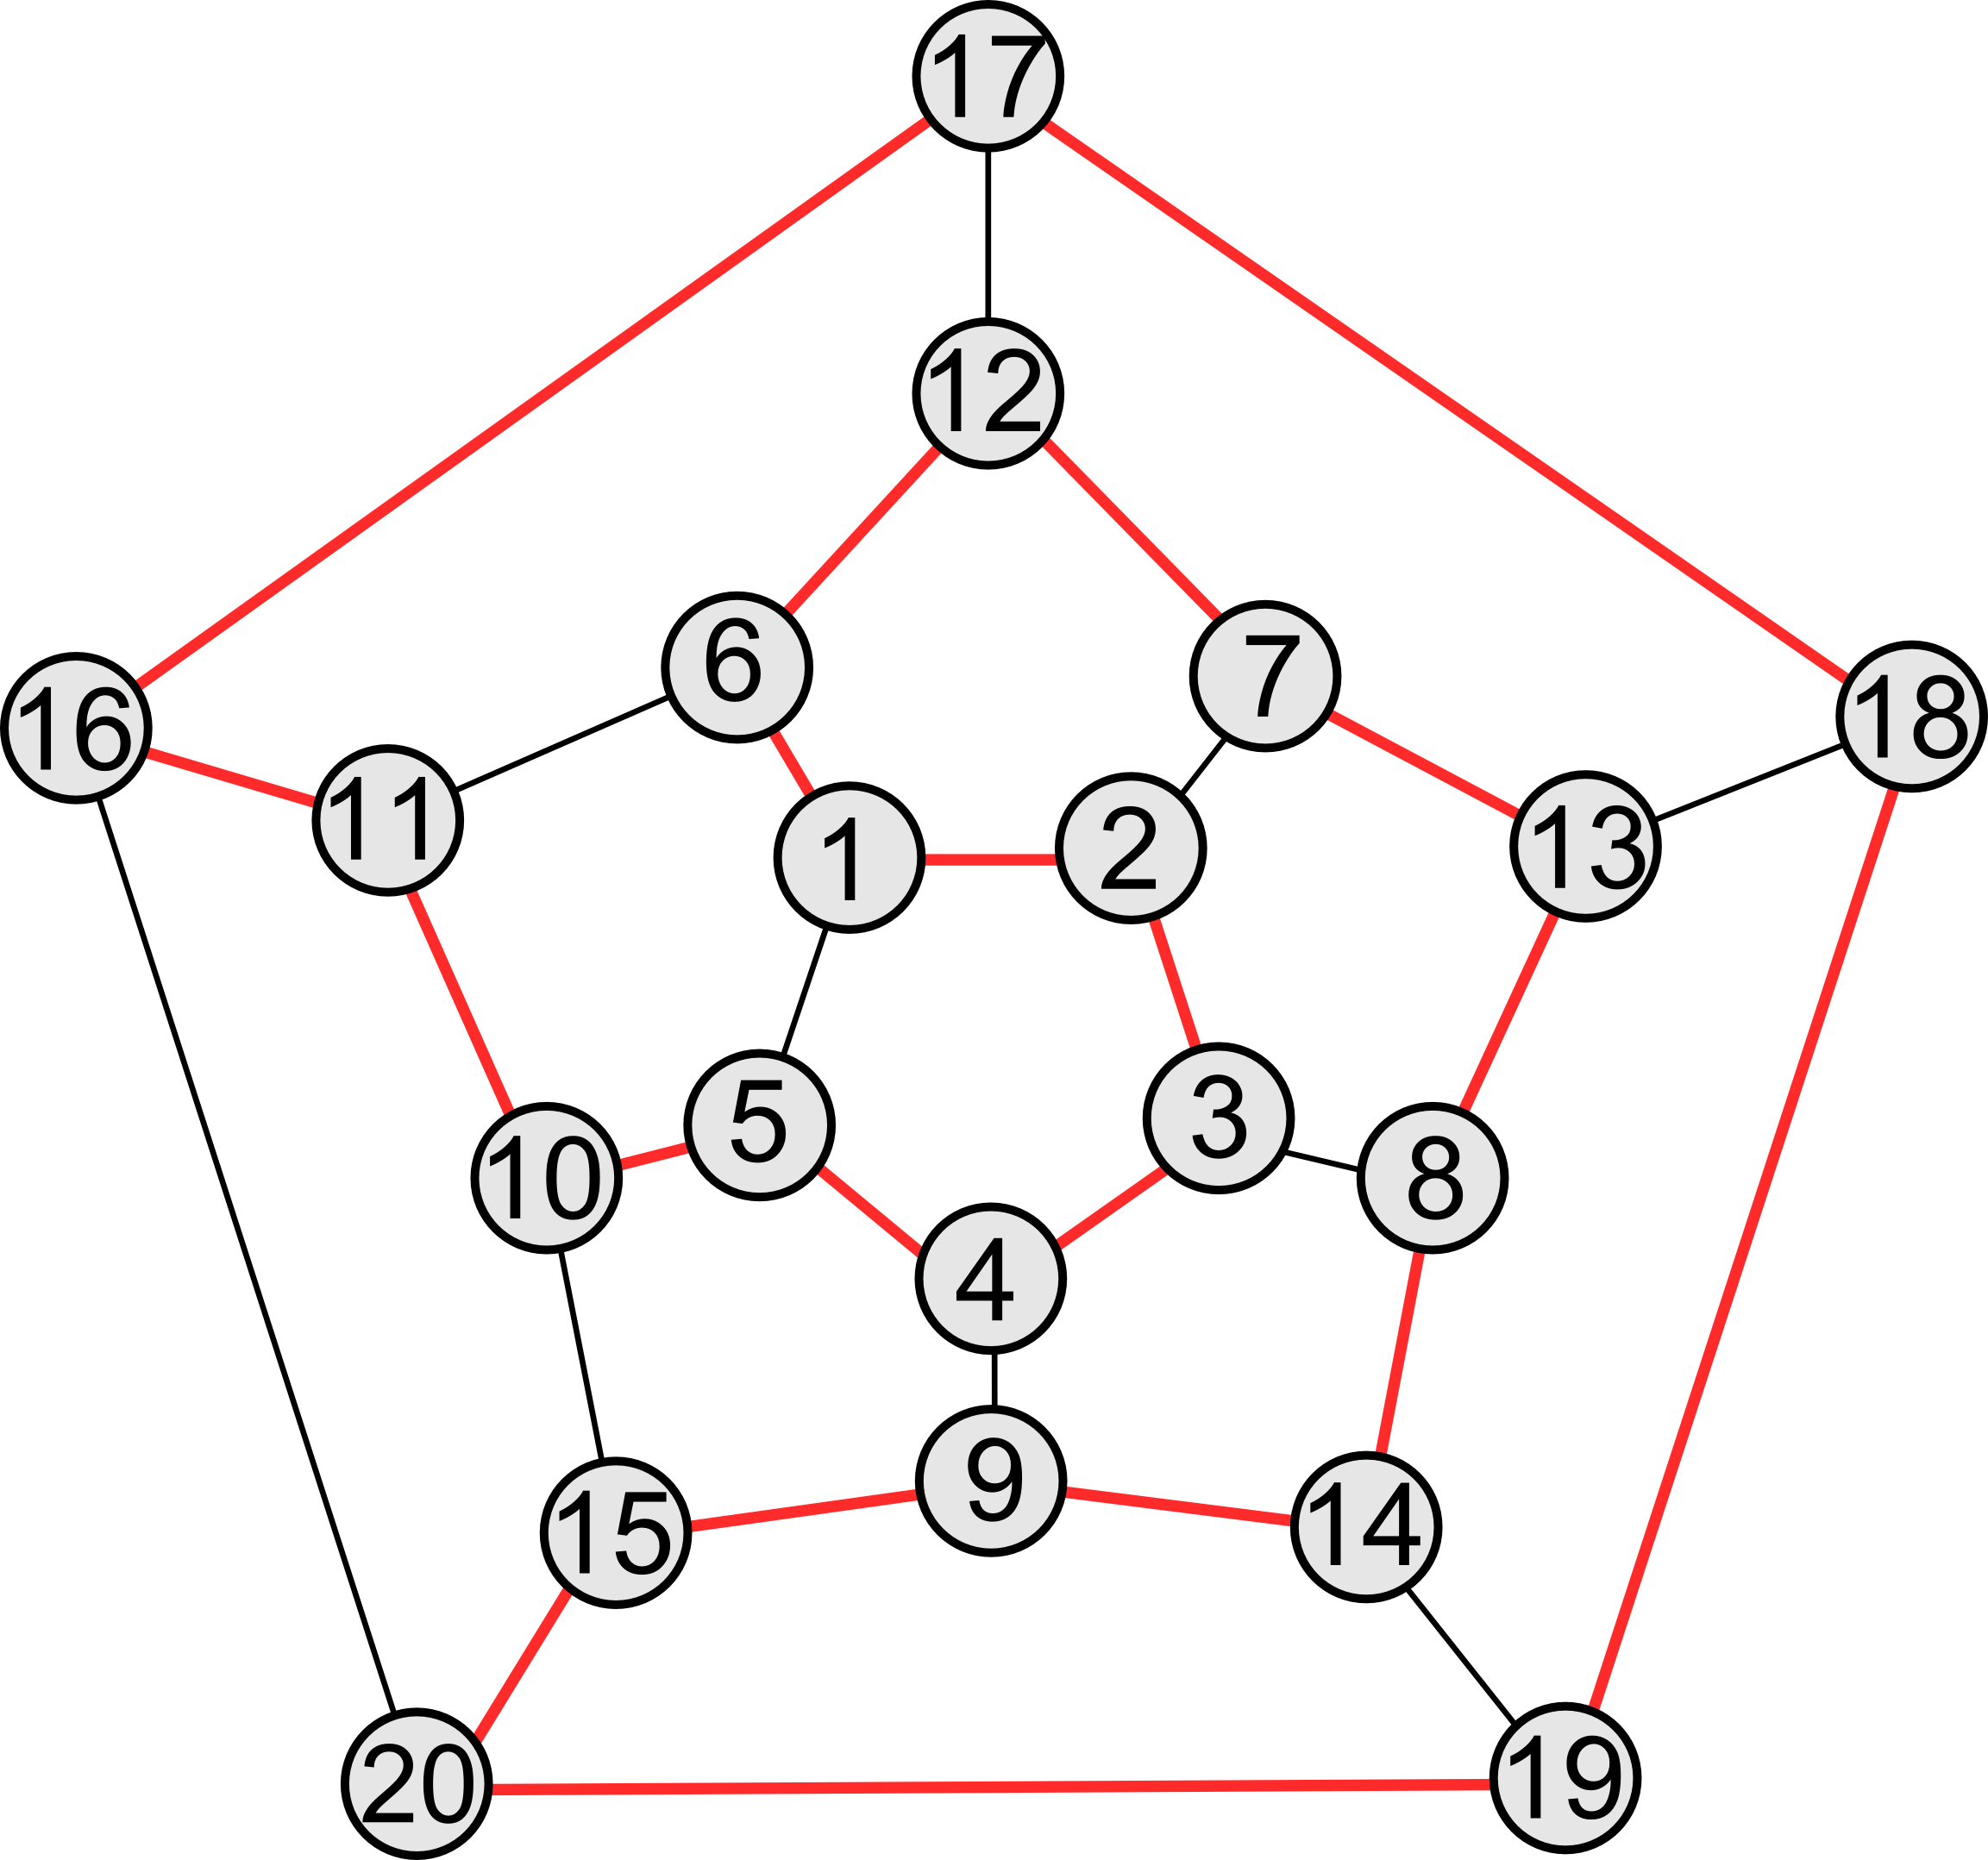
\includegraphics[scale=0.45]{hamiltonial.png}
\end{frame}

\begin{frame}{Examples}
\begin{itemize}
\item $AtLeastOne(x_1, \dots, x_n)$
\item $AtMostOne(x_1, \dots, x_n)$
\item Lazy approach
\end{itemize}
\end{frame}

\begin{frame}{}
\begin{itemize}
\item $(x = 4) \wedge ((y = 7) \vee (x = y))$
\item $(x + y = 3) \wedge (y - z = 7) \wedge (z * 2 = 4)$
\item $(lenght(s) = 3) \wedge (s[0] = 'a') \wedge (s[1] = 'b') \wedge (s[2] = 'c')$
\end{itemize}
\end{frame}


\begin{frame}{Definitions}
\begin{block}{First-order logic}
\begin{itemize}
\item Variables: a set of variables
\item Logical symbols: the standard Boolean connectives (e.g., $\wedge, \vee, \lnot$), quantifiers ($\exists$ and $\forall$), and parentheses
\item Nonlogical symbols: function, predicate, and constant symbols
\item Syntax: rules for constructing formulas. Formulas adhering to these rules are said to be well formed
\end{itemize}
\end{block}
\begin{block}{}
\begin{itemize}
\item A domain
\item An interpretation of the nonlogical symbols, in the form of a mapping from each function and predicate symbol to a function and a predicate, respectively, and an assignment of a domain element to each of the constant symbols
\item An assignment of a domain element to each of the free (unquantified) variables
\end{itemize}
\end{block}
\end{frame}

\begin{frame}{Definitions}
\begin{block}{Satisfiability}
The formula $\varphi$ is satisfiable if and only if there exists a structure under which the formula is true.
\end{block}
\end{frame}

\begin{frame}{Expressiveness}
\begin{block}{}
Theory A is more expressive than theory B if every language that can be defined by a B-formula can also be defined by an A-formula, and there exists at least one language definable by an A-formula that cannot be defined by a B-formula. We denote the fact that theory B is less expressive than theory A by B $\prec$ A.
\end{block}
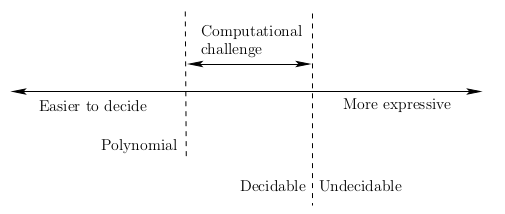
\includegraphics[scale=0.5]{expressiveness.png}
\end{frame}

\begin{frame}{logics}
\begin{itemize}
\item Propositional Logic
\item Equalities and Uninterpreted Functions
\item Linear Arithmetic
\item Bit Vectors
\item Arrays
\item Pointer Logic
\end{itemize}
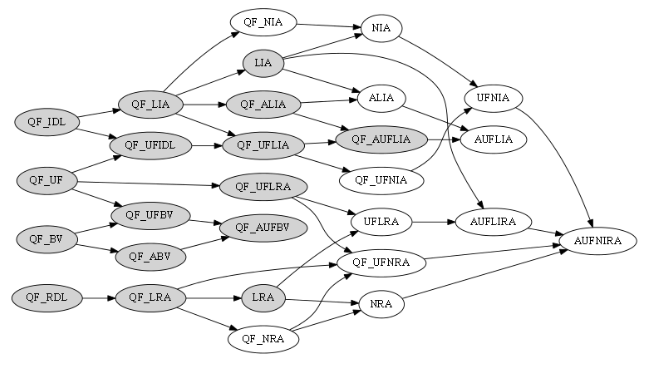
\includegraphics[scale=0.4]{logics.png}
\end{frame}

\begin{frame}{Solvers}
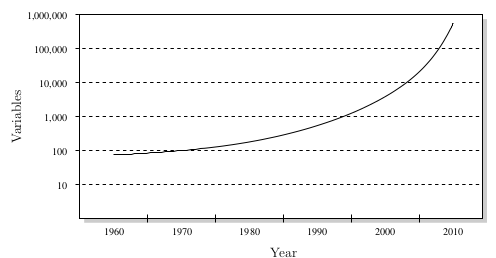
\includegraphics[scale=0.6]{SAT_results0.png}
\end{frame}

\begin{frame}{Solvers}
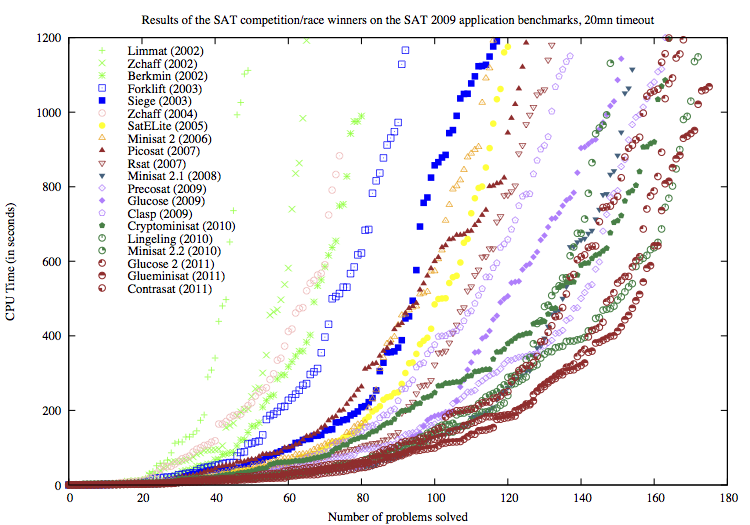
\includegraphics[scale=0.4]{SAT_results1.png}
\end{frame}

\begin{frame}{Solvers}
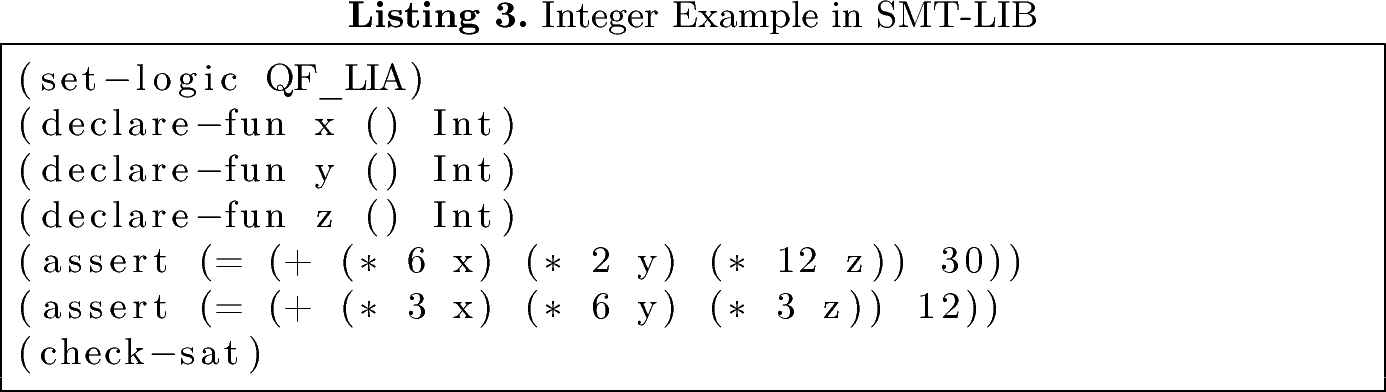
\includegraphics[scale=1.0]{SMT-LIB.png}
\end{frame}

\begin{frame}{DIMACS format}
\begin{itemize}
\item $(a \vee b \vee \lnot c) \wedge (\lnot a \vee \lnot b \vee c) \wedge (b \vee c \vee \lnot d)$
\item c example\newline
p cnf 4 3\newline
1 2 -3 0\newline
-1 -2 3 0\newline
2 3 -4 0\newline
\end{itemize}
\end{frame}

\begin{frame}{Additional materials}
\begin{itemize}
\item Decision Procedures An Algorithmic Point of View, Daniel Kroening, Ofer Strichman
\item Handbook of satisfiability, Edmund Clarke
\item The art of Computer Programming, volume 4, part 6, Donald Knuth
\end{itemize}
\end{frame}

\begin{frame}
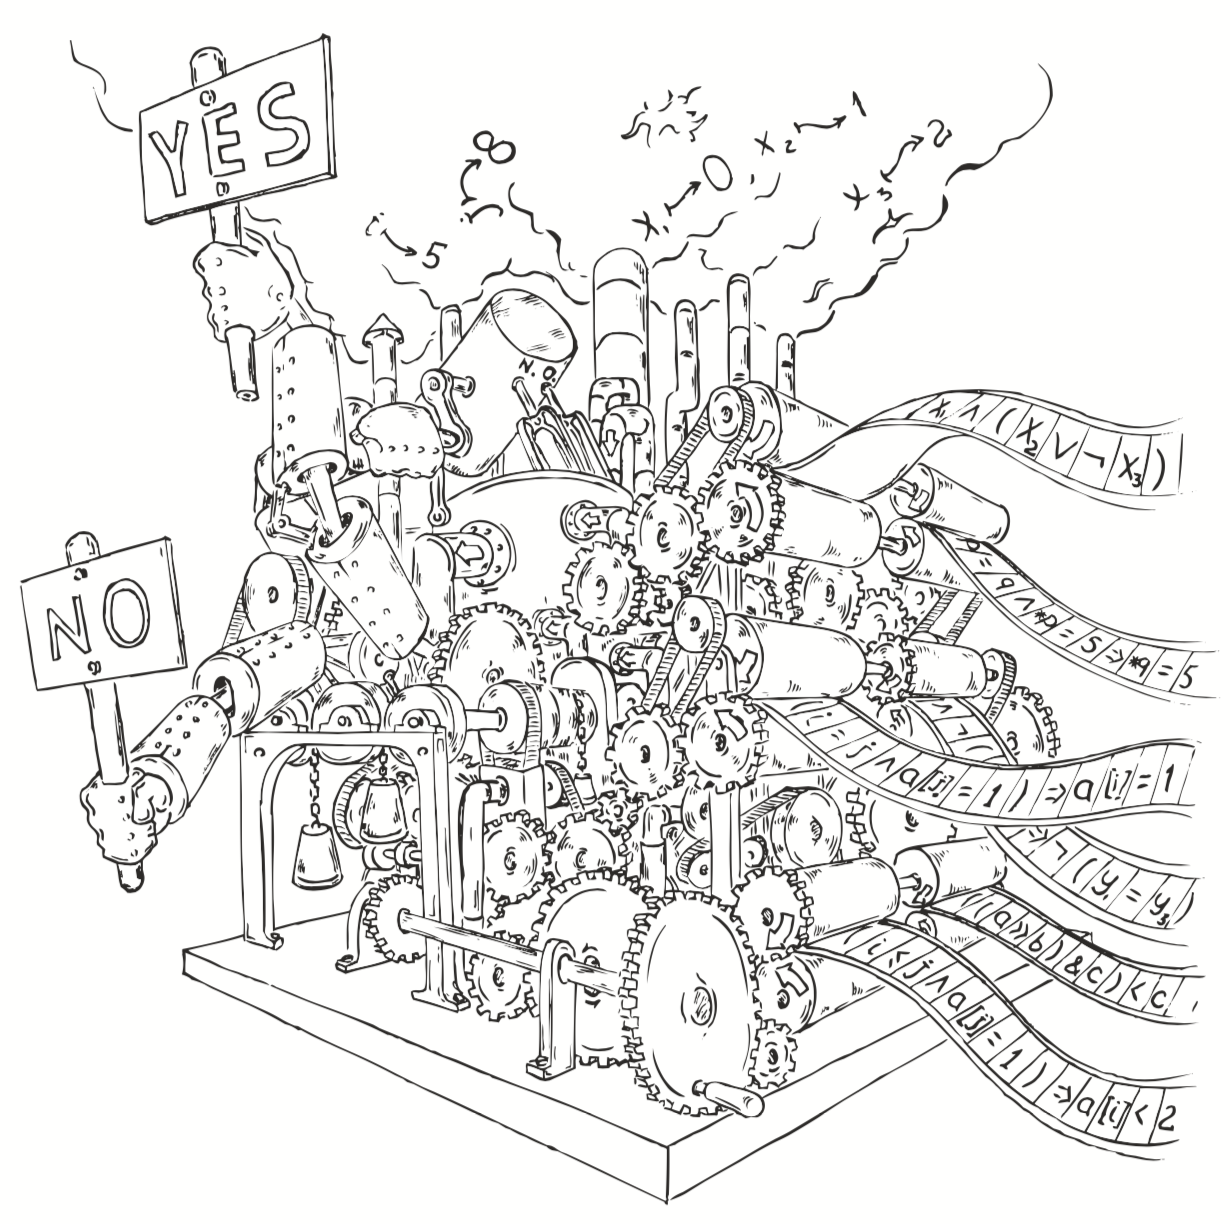
\includegraphics[scale=0.5]{../decision-procedure.png}
\end{frame}

\end{document}
